
%% bare_conf.tex
%% V1.3
%% 2007/01/11
%% by Michael Shell
%% See:
%% http://www.michaelshell.org/
%% for current contact information.
%%
%% This is a skeleton file demonstrating the use of IEEEtran.cls
%% (requires IEEEtran.cls version 1.7 or later) with an IEEE conference paper.
%%
%% Support sites:
%% http://www.michaelshell.org/tex/ieeetran/
%% http://www.ctan.org/tex-archive/macros/latex/contrib/IEEEtran/
%% and
%% http://www.ieee.org/

%%*************************************************************************
%% Legal Notice:
%% This code is offered as-is without any warranty either expressed or
%% implied; without even the implied warranty of MERCHANTABILITY or
%% FITNESS FOR A PARTICULAR PURPOSE! 
%% User assumes all risk.
%% In no event shall IEEE or any contributor to this code be liable for
%% any damages or losses, including, but not limited to, incidental,
%% consequential, or any other damages, resulting from the use or misuse
%% of any information contained here.{
%%
%% All comments are the opinions of their respective authors and are not
%% necessarily endorsed by the IEEE.
%%
%% This work is distributed under the LaTeX Project Public License (LPPL)
%% ( http://www.latex-project.org/ ) version 1.3, and may be freely used,
%% distributed and modified. A copy of the LPPL, version 1.3, is included
%% in the base LaTeX documentation of all distributions of LaTeX released
%% 2003/12/01 or later.
%% Retain all contribution notices and credits.
%% ** Modified files should be clearly indicated as such, including  **
%% ** renaming them and changing author support contact information. **
%%
%% File list of work: IEEEtran.cls, IEEEtran_HOWTO.pdf, bare_adv.tex,
%%                    bare_conf.tex, bare_jrnl.tex, bare_jrnl_compsoc.tex
%%*************************************************************************

% *** Authors should verify (and, if needed, correct) their LaTeX system  ***
% *** with the testflow diagnostic prior to trusting their LaTeX platform ***
% *** with production work. IEEE's font choices can trigger bugs that do  ***
% *** not appear when using other class files.                            ***
% The testflow support page is at:
% http://www.michaelshell.org/tex/testflow/



% Note that the a4paper option is mainly intended so that authors in
% countries using A4 can easily print to A4 and see how their papers will
% look in print - the typesetting of the document will not typically be
% affected with changes in paper size (but the bottom and side margins will).
% Use the testflow package mentioned above to verify correct handling of
% both paper sizes by the user's LaTeX system.
%
% Also note that the "draftcls" or "draftclsnofoot", not "draft", option
% should be used if it is desired that the figures are to be displayed in
% draft mode.
%
\documentclass[conference]{IEEEtran}
% Add the compsoc option for Computer Society conferences.
%
% If IEEEtran.cls has not been installed into the LaTeX system files,
% manually specify the path to it like:
% \documentclass[conference]{../sty/IEEEtran}





% Some very useful LaTeX packages include:
% (uncomment the ones you want to load)


% *** MISC UTILITY PACKAGES ***
%
%\usepackage{ifpdf}
% Heiko Oberdiek's ifpdf.sty is very useful if you need conditional
% compilation based on whether the output is pdf or dvi.
% usage:
% \ifpdf
%   % pdf code
% \else
%   % dvi code
% \fi
% The latest version of ifpdf.sty can be obtained from:
% http://www.ctan.org/tex-archive/macros/latex/contrib/oberdiek/
% Also, note that IEEEtran.cls V1.7 and later provides a builtin
% \ifCLASSINFOpdf conditional that works the same way.
% When switching from latex to pdflatex and vice-versa, the compiler may
% have to be run twice to clear warning/error messages.






% *** CITATION PACKAGES ***
%
%\usepackage{cite}
% cite.sty was written by Donald Arseneau
% V1.6 and later of IEEEtran pre-defines the format of the cite.sty package
% \cite{} output to follow that of IEEE. Loading the cite package will
% result in citation numbers being automatically sorted and properly
% "compressed/ranged". e.g., [1], [9], [2], [7], [5], [6] without using
% cite.sty will become [1], [2], [5]--[7], [9] using cite.sty. cite.sty's
% \cite will automatically add leading space, if needed. Use cite.sty's
% noadjust option (cite.sty V3.8 and later) if you want to turn this off.
% cite.sty is already installed on most LaTeX systems. Be sure and use
% version 4.0 (2003-05-27) and later if using hyperref.sty. cite.sty does
% not currently provide for hyperlinked citations.
% The latest version can be obtained at:
% http://www.ctan.org/tex-archive/macros/latex/contrib/cite/
% The documentation is contained in the cite.sty file itself.






% *** GRAPHICS RELATED PACKAGES ***
%
\ifCLASSINFOpdf
  % \usepackage[pdftex]{graphicx}
  % declare the path(s) where your graphic files are
  % \graphicspath{{../pdf/}{../jpeg/}}
  % and their extensions so you won't have to specify these with
  % every instance of \includegraphics
  % \DeclareGraphicsExtensions{.pdf,.jpeg,.png}
\else
  % or other class option (dvipsone, dvipdf, if not using dvips). graphicx
  % will default to the driver specified in the system graphics.cfg if no
  % driver is specified.
  % \usepackage[dvips]{graphicx}
  % declare the path(s) where your graphic files are
  % \graphicspath{{../eps/}}
  % and their extensions so you won't have to specify these with
  % every instance of \includegraphics
  % \DeclareGraphicsExtensions{.eps}
\fi
% graphicx was written by David Carlisle and Sebastian Rahtz. It is
% required if you want graphics, photos, etc. graphicx.sty is already
% installed on most LaTeX systems. The latest version and documentation can
% be obtained at: 
% http://www.ctan.org/tex-archive/macros/latex/required/graphics/
% Another good source of documentation is "Using Imported Graphics in
% LaTeX2e" by Keith Reckdahl which can be found as epslatex.ps or
% epslatex.pdf at: http://www.ctan.org/tex-archive/info/
%
% latex, and pdflatex in dvi mode, support graphics in encapsulated
% postscript (.eps) format. pdflatex in pdf mode supports graphics
% in .pdf, .jpeg, .png and .mps (metapost) formats. Users should ensure
% that all non-photo figures use a vector format (.eps, .pdf, .mps) and
% not a bitmapped formats (.jpeg, .png). IEEE frowns on bitmapped formats
% which can result in "jaggedy"/blurry rendering of lines and letters as
% well as large increases in file sizes.
%
% You can find documentation about the pdfTeX application at:
% http://www.tug.org/applications/pdftex


\usepackage{graphicx}


% *** MATH PACKAGES ***
%
%\usepackage[cmex10]{amsmath}
% A popular package from the American Mathematical Society that provides
% many useful and powerful commands for dealing with mathematics. If using
% it, be sure to load this package with the cmex10 option to ensure that
% only type 1 fonts will utilized at all point sizes. Without this option,
% it is possible that some math symbols, particularly those within
% footnotes, will be rendered in bitmap form which will result in a
% document that can not be IEEE Xplore compliant!
%
% Also, note that the amsmath package sets \interdisplaylinepenalty to 10000
% thus preventing page breaks from occurring within multiline equations. Use:
%\interdisplaylinepenalty=2500
% after loading amsmath to restore such page breaks as IEEEtran.cls normally
% does. amsmath.sty is already installed on most LaTeX systems. The latest
% version and documentation can be obtained at:
% http://www.ctan.org/tex-archive/macros/latex/required/amslatex/math/





% *** SPECIALIZED LIST PACKAGES ***
%
%\usepackage{algorithmic}
% algorithmic.sty was written by Peter Williams and Rogerio Brito.
% This package provides an algorithmic environment fo describing algorithms.
% You can use the algorithmic environment in-text or within a figure
% environment to provide for a floating algorithm. Do NOT use the algorithm
% floating environment provided by algorithm.sty (by the same authors) or
% algorithm2e.sty (by Christophe Fiorio) as IEEE does not use dedicated
% algorithm float types and packages that provide these will not provide
% correct IEEE style captions. The latest version and documentation of
% algorithmic.sty can be obtained at:
% http://www.ctan.org/tex-archive/macros/latex/contrib/algorithms/
% There is also a support site at:
% http://algorithms.berlios.de/index.html
% Also of interest may be the (relatively newer and more customizable)
% algorithmicx.sty package by Szasz Janos:
% http://www.ctan.org/tex-archive/macros/latex/contrib/algorithmicx/




% *** ALIGNMENT PACKAGES ***
%
%\usepackage{array}
% Frank Mittelbach's and David Carlisle's array.sty patches and improves
% the standard LaTeX2e array and tabular environments to provide better
% appearance and additional user controls. As the default LaTeX2e table
% generation code is lacking to the point of almost being broken with
% respect to the quality of the end results, all users are strongly
% advised to use an enhanced (at the very least that provided by array.sty)
% set of table tools. array.sty is already installed on most systems. The
% latest version and documentation can be obtained at:
% http://www.ctan.org/tex-archive/macros/latex/required/tools/


%\usepackage{mdwmath}
%\usepackage{mdwtab}
% Also highly recommended is Mark Wooding's extremely powerful MDW tools,
% especially mdwmath.sty and mdwtab.sty which are used to format equations
% and tables, respectively. The MDWtools set is already installed on most
% LaTeX systems. The lastest version and documentation is available at:
% http://www.ctan.org/tex-archive/macros/latex/contrib/mdwtools/


% IEEEtran contains the IEEEeqnarray family of commands that can be used to
% generate multiline equations as well as matrices, tables, etc., of high
% quality.


%\usepackage{eqparbox}
% Also of notable interest is Scott Pakin's eqparbox package for creating
% (automatically sized) equal width boxes - aka "natural width parboxes".
% Available at:
% http://www.ctan.org/tex-archive/macros/latex/contrib/eqparbox/





% *** SUBFIGURE PACKAGES ***
%\usepackage[tight,footnotesize]{subfigure}
% subfigure.sty was written by Steven Douglas Cochran. This package makes it
% easy to put subfigures in your figures. e.g., "Figure 1a and 1b". For IEEE
% work, it is a good idea to load it with the tight package option to reduce
% the amount of white space around the subfigures. subfigure.sty is already
% installed on most LaTeX systems. The latest version and documentation can
% be obtained at:
% http://www.ctan.org/tex-archive/obsolete/macros/latex/contrib/subfigure/
% subfigure.sty has been superceeded by subfig.sty.



%\usepackage[caption=false]{caption}
%\usepackage[font=footnotesize]{subfig}
% subfig.sty, also written by Steven Douglas Cochran, is the modern
% replacement for subfigure.sty. However, subfig.sty requires and
% automatically loads Axel Sommerfeldt's caption.sty which will override
% IEEEtran.cls handling of captions and this will result in nonIEEE style
% figure/table captions. To prevent this problem, be sure and preload
% caption.sty with its "caption=false" package option. This is will preserve
% IEEEtran.cls handing of captions. Version 1.3 (2005/06/28) and later 
% (recommended due to many improvements over 1.2) of subfig.sty supports
% the caption=false option directly:
%\usepackage[caption=false,font=footnotesize]{subfig}
%
% The latest version and documentation can be obtained at:
% http://www.ctan.org/tex-archive/macros/latex/contrib/subfig/
% The latest version and documentation of caption.sty can be obtained at:
% http://www.ctan.org/tex-archive/macros/latex/contrib/caption/




% *** FLOAT PACKAGES ***
%
%\usepackage{fixltx2e}
% fixltx2e, the successor to the earlier fix2col.sty, was written by
% Frank Mittelbach and David Carlisle. This package corrects a few problems
% in the LaTeX2e kernel, the most notable of which is that in current
% LaTeX2e releases, the ordering of single and double column floats is not
% guaranteed to be preserved. Thus, an unpatched LaTeX2e can allow a
% single column figure to be placed prior to an earlier double column
% figure. The latest version and documentation can be found at:
% http://www.ctan.org/tex-archive/macros/latex/base/



%\usepackage{stfloats}
% stfloats.sty was written by Sigitas Tolusis. This package gives LaTeX2e
% the ability to do double column floats at the bottom of the page as well
% as the top. (e.g., "\begin{figure*}[!b]" is not normally possible in
% LaTeX2e). It also provides a command:
%\fnbelowfloat
% to enable the placement of footnotes below bottom floats (the standard
% LaTeX2e kernel puts them above bottom floats). This is an invasive package
% which rewrites many portions of the LaTeX2e float routines. It may not work
% with other packages that modify the LaTeX2e float routines. The latest
% version and documentation can be obtained at:
% http://www.ctan.org/tex-archive/macros/latex/contrib/sttools/
% Documentation is contained in the stfloats.sty comments as well as in the
% presfull.pdf file. Do not use the stfloats baselinefloat ability as IEEE
% does not allow \baselineskip to stretch. Authors submitting work to the
% IEEE should note that IEEE rarely uses double column equations and
% that authors should try to avoid such use. Do not be tempted to use the
% cuted.sty or midfloat.sty packages (also by Sigitas Tolusis) as IEEE does
% not format its papers in such ways.





% *** PDF, URL AND HYPERLINK PACKAGES ***
%
%\usepackage{url}
% url.sty was written by Donald Arseneau. It provides better support for
% handling and breaking URLs. url.sty is already installed on most LaTeX
% systems. The latest version can be obtained at:
% http://www.ctan.org/tex-archive/macros/latex/contrib/misc/
% Read the url.sty source comments for usage information. Basically,
% \url{my_url_here}.





% *** Do not adjust lengths that control margins, column widths, etc. ***
% *** Do not use packages that alter fonts (such as pslatex).         ***
% There should be no need to do such things with IEEEtran.cls V1.6 and later.
% (Unless specifically asked to do so by the journal or conference you plan
% to submit to, of course. )
\usepackage{hyperref}
%\usepackage[backref]{hyperref} % to see how much/where references are used
\usepackage{cite}


\newcounter{questionno}
\addtocounter{questionno}{1}
%
%\newcommand{\mytodo}[1]{\textbf{[[#1]]}}
%
\newcommand{\subsubsectionx}[1]{{\em {\arabic{questionno}) #1}}
	\addtocounter{questionno}{1}
	}


\begin{document}
%
% paper title
% can use linebreaks \\ within to get better formatting as desired
%\title{AI as Game Producer}
\title{AI for Game Production}

% author names and affiliations
% use a multiple column layout for up to three different
% affiliations
\author{
\IEEEauthorblockN{Mark Owen Riedl}
\IEEEauthorblockA{School of Interactive Computing\\
Georgia Institute of Technology\\
riedl@cc.gatech.edu}
\and
\IEEEauthorblockN{Alexander Zook}
\IEEEauthorblockA{School of Interactive Computing\\
Georgia Institute of Technology\\
a.zook@gatech.edu}
}

% conference papers do not typically use \thanks and this command
% is locked out in conference mode. If really needed, such as for
% the acknowledgment of grants, issue a \IEEEoverridecommandlockouts
% after \documentclass

% for over three affiliations, or if they all won't fit within the width
% of the page, use this alternative format:
% 
%\author{\IEEEauthorblockN{Michael Shell\IEEEauthorrefmark{1},
%Homer Simpson\IEEEauthorrefmark{2},
%James Kirk\IEEEauthorrefmark{3}, 
%Montgomery Scott\IEEEauthorrefmark{3} and
%Eldon Tyrell\IEEEauthorrefmark{4}}
%\IEEEauthorblockA{\IEEEauthorrefmark{1}School of Electrical and Computer Engineering\\
%Georgia Institute of Technology,
%Atlanta, Georgia 30332--0250\\ Email: see http://www.michaelshell.org/contact.html}
%\IEEEauthorblockA{\IEEEauthorrefmark{2}Twentieth Century Fox, Springfield, USA\\
%Email: homer@thesimpsons.com}
%\IEEEauthorblockA{\IEEEauthorrefmark{3}Starfleet Academy, San Francisco, California 96678-2391\\
%Telephone: (800) 555--1212, Fax: (888) 555--1212}
%\IEEEauthorblockA{\IEEEauthorrefmark{4}Tyrell Inc., 123 Replicant Street, Los Angeles, California 90210--4321}}




% use for special paper notices
%\IEEEspecialpapernotice{(Invited Paper)}




% make the title area
\maketitle


\begin{abstract}
%\boldmath
A number of changes are occurring in the field of computer game development:
persistent online games, digital distribution platforms and portals, social and mobile games, and the emergence of new business models have pushed game development to put heavier emphasis on the live operation of games.
Artificial intelligence has long been an important part of game development practices.
The forces of change in the industry present an opportunity for Game AI to have new and profound impact on game production practices. 
%% compared to earlier processes aimed to deliver a boxed product.
%Game AI encompasses tools for creating interactive entertainment experiences and as such should adapt to meet this new environment.
%%``Game AI 1.0'' treated game AI agents as actors within games and ``Game AI 2.0'' targeted AI agents acting as designers of single games.
%%In contrast, ``Game AI 3.0'' considers game AI agents as producers responsible for managing a long-running set of live games, their player communities, and real-world context.
Specifically, Game AI agents should act as ``producers'' responsible for managing a long-running set of live games, their player communities, and real-world context.
We characterize a confluence of four major forces at play in the games industry today, together producing a wealth of data that opens unique research opportunities and challenges for Game AI in game production.
%Combined, these four forces are driving the need for Game AI systems that act as Producers to use this data to 
We enumerate 12 new research areas spawned by these forces and steps toward how they can be addressed by data-driven Game AI Producers.
\end{abstract}
% IEEEtran.cls defaults to using nonbold math in the Abstract.
% This preserves the distinction between vectors and scalars. However,
% if the conference you are submitting to favors bold math in the abstract,
% then you can use LaTeX's standard command \boldmath at the very start
% of the abstract to achieve this. Many IEEE journals/conferences frown on
% math in the abstract anyway.

% no keywords




% For peer review papers, you can put extra information on the cover
% page as needed:
% \ifCLASSOPTIONpeerreview
% \begin{center} \bfseries EDICS Category: 3-BBND \end{center}
% \fi
%
% For peerreview papers, this IEEEtran command inserts a page break and
% creates the second title. It will be ignored for other modes.
\IEEEpeerreviewmaketitle



%\section{Introduction}
%% no \IEEEPARstart
%This demo file is intended to serve as a ``starter file''
%for IEEE conference papers produced under \LaTeX\ using
%IEEEtran.cls version 1.7 and later.
%% You must have at least 2 lines in the paragraph with the drop letter
%% (should never be an issue)

\section{Introduction}
% intro 4 forces
Over the past several years the game industry has undergone a series of major changes. 
The increasing prominence of persistent online games, digital distribution platforms and portals, mobile and social games, and the emergence of new business models have all changed fundamental aspects of making and playing games. 
Developers increasingly focus on the live operation of a game, rather than creating a boxed and finalized product.
Players are more diverse, have access to games in more places and at more times, and produce more data and content for developers to leverage than ever before. Across these changes four forces have come to the fore:
\begin{enumerate}
\item Games and cross-game play is increasingly persistent and presenting longer-term experiences %;
\item Game developers are starting to see their game titles as an ecosystem wherein players may move from game to game %;
\item Player communities and social gameplay have gained prominence
%Greater emphasis on community and social gaming %;
\item Developers and players have a growing interest in coupling the real world and virtual world(s) %; and
%\item Developers are embracing end-user generated content %. 
\end{enumerate}
\noindent
Some of these forces have been around for a number of years, while others are just beginning to emerge.
The consequence of these forces is a profound opportunity for Artificial Intelligence (AI), Computational Intelligence (CI), and Machine Learning (ML) in games (collectively referred to as {\em Game AI}) to play an even greater role in the development of computer games and the delivery of engaging real-time experiences to players. 

Through these forces we see an opportunity for Game AI to address new research questions that have the potential to dramatically impact game development practices.
%
The most significant consequence of the shifting landscape of computer game development is the generation of massive amounts of data. 
Researchers and game developers can leverage this data in a new paradigm of data-driven Game AI focused on how to use these sources of data to 
%address novel research questions that emerge within these domains. 
improve game development practices and to deliver more engaging experiences.
However, we are not merely advocating that researchers and game developers adopt data-driven analogues to existing Game AI practices (although that would be a worthy endeavor).
%Instead, we are proposing that the massive amounts of data now available, coupled with a new understanding of the forces driving game development, have opened up a number of new, exciting research questions. 
Instead, we are proposing that the market forces enumerated above are forcing the industry to change how they think about game development processes.
The modern development environment presents significant challenges to scalability---of both the practice of creating games and also the size and scope of games themselves---that are readily addressed by artificial intelligent, computational intelligence, and machine learning research.

% % three stakeholders: players, designers, producers
Game AI was initially about supporting the interaction between player and the game itself.
% (which we dub {\em Game AI 1.0}).
Recently there has been a push for procedural content generation as a means to support and augment the game developer on a game by game basis.
% ({\em Game AI 2.0}) 
%
In this paper, we present our desiderata on the future of Game AI
%---{\em Game AI 3.0}---
in which intelligent systems support the entire game production pipeline from game creation to live operation, and across a number of games and game genres.
%In particular we focus on the research questions that may soon be addressed, with pointers to places where we see initial steps toward Game AI 3.0 problems being taken. 
%We will first describe the shifting landscape of computer game development that has driven our desiderata and the historical precedents behind it (what we call {\em Game AI 1.0} and {\em Game AI 2.0}). 
This perspective of Game AI 
%as ``producer'' 
for production
does not supplant or replace prior perspectives on Game AI, but presents a new lens through which to see an expanded role for Game AI in computer game production. 
We will enumerate 12 novel research questions that arise when considering the role of AI as Producer and discuss steps toward how these challenges may be addressed. 
%We 
%and present some of the steps researchers and game developers are already beginning to take along this direction. 
%In the course of our desiderata, 
%\mytodo{then what?}

%%%%%%%%%%%%%%%%%%%%%%%%%%

\section{The Shifting Landscape of Game Development}

In this section, we enumerate some of the prominent new forces that are shaping the way that computer game development companies create games. 
Many of these forces have arisen as a confluence of advances in computing technology and market forces that result from a maturation of the computer game industry.

%\begin{description}
%\item[\textbf{persistent games}] \hfill \\ 
%{\bf Persistent Games}
\subsubsection{Persistent Games} 
The rise of Massively Multiplayer Online Games (MMOGs), social games, online game portals and long-term or recurring game experiences is creating long-term data on players within games. 
Many games have players join, play over long periods of time, and potentially rejoin at later times. 
Developers are increasingly pressed to develop content that provides long-term engagement with a game, rather than a closed experience with clear beginning and end.

%\item[\textbf{ecosystem of games}] \hfill \\ 
%{\bf Ecosystem of Games}
\subsubsection{Ecosystem of Games}
Developers have a wider variety of tools to build games and lowered barriers to distributing games to new users through digital platforms and online portals. 
Together this puts greater emphasis on keeping players engaged within an ecosystem of games from a single developer, rather than focusing on experiences only within one game. 
Developers are driven to provide new content of multiple kinds (including meta-game objectives) that engage players across games. 
The growing diversity of game players has led to additional emphasis on ensuring an ecosystem of games provides a diverse range of experiences.
%, rather than create a kind of experience within a single game.

\begin{figure*}
\centering
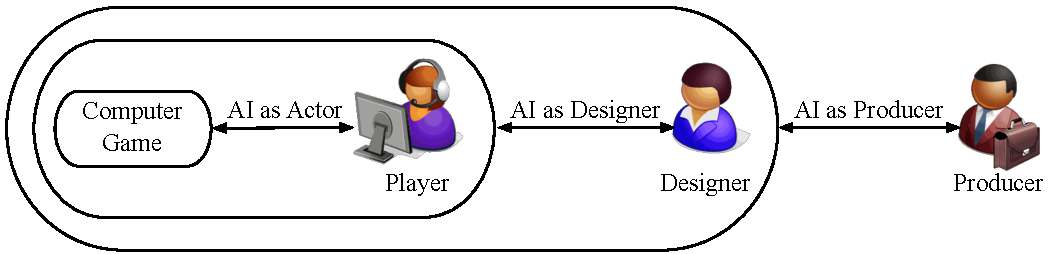
\includegraphics[scale=0.7, natwidth=100, natheight=100]{metaphor.pdf}
%\caption{Three paradigms of Game AI. The {\em AI as Actor} paradigm describes how AI mediates between the user and the game itself. The {\em AI as Designer} paradigm describes how AI mediates between a single game developer and the human-computer system of player and game. The {\em AI as Producer} is a new paradigm describing how AI mediates between producers and many systems of designers, users, and games.}
\caption{Three roles of Game AI and their human stakeholders.
{\em AI as Actor} describes how AI mediates between the player and the game itself. 
{\em AI as Designer} describes how AI mediates between a single game designer and the human-computer system of player and game. 
{\em AI as Producer} is a new role describing how AI mediates between producers and many systems of designers, users, and games.
}
\label{fig:metaphor}
\end{figure*}

%\item[\textbf{community}] \hfill \\ 
%{\bf Player Communities}
\subsubsection{Player Communities}
Player communities have emerged as a major driving force for the success (and failure) of games. 
Players generate a mass of content from reviews and walkthoughs through add-ons and full game modifications.
Continually engaging communities, supporting player socializing within the community, managing how players impact ones another's experiences (positively and negatively), and leveraging user-generated content are growing concerns.


%\item[\textbf{real-virtual coupling}] \hfill \\ 
%{\bf Coupling of Real and Virtual Worlds}
\subsubsection{Coupling of Real and Virtual Worlds}
Games are more widely adopting ways to connect to the real world. 
Sensing systems from the Kinect and Wiimote to mobile phone GPS provide more data on players' real-world environment. 
Output modalities from second screen experiences and mobile phone augmented reality to virtual reality are emerging as new ways to view game content. 
At the same time these technologies have introduced a host of challenges around how games can interface with and use this real-world context and respond to more unstructured types of information.

%%\item[\textbf{user-generated content}] \hfill \\ 
%{\bf User-Generated Content}
%Games have historically provided many opportunities for modification (``modding'') and some degree of editing. Recently, however, this force has become a driving aspect of long-term success, exemplified by games including Minecraft, LittleBigPlanet, and Second Life. Developers are increasingly pressured to provide tools for users to create content, manage that content, and promote content within game communities.
%%\end{description}
%% data-centric consequences


Each of these forces presents new opportunities to solve problems of real-world applicability to game developers.
A side effect of each of these forces is the massive amounts of data being generated about game players.
While it is not necessarily the case that new research problems will require data-driven AI, CI, and ML techniques, we see this data as a tool for tackling real-world game development problems.
%Each of these forces provides massive amounts of data to game developers. 
%Research in game AI can leverage this data in a new paradigm of data-driven game AI focused on how to use these sources of data to address novel research questions that emerge within these domains. [weak statement, want something stronger about need to respond]

%%%%%%%%%%%%%%%%%%%%%%%%%%%


\section{Background: Three Roles of Game AI}

In 2001, Laird and van Lent \cite{laird2001:gameai} put forth their seminal argument for AI in computer games as an academic pursuit. 
They specifically argued that the pursuit of ``human-level'' AI systems could use computer games as testbeds for research because games were intermediate environments between the toy domains researchers had been using and the full complexity of the real world.
While this opened Game AI as an academic endeavor, the automation of various aspects of computer games has been a part of the industrial practice of creating commercial computer games since the beginning. 

{\em Game AI} has come to refer to the set of tools---algorithms and representations---developed specifically to aid the creation and management of interactive, real-time, digital entertainment experiences.
While games are played by humans, there are a number of aspects of the game playing experience that must be automated: roles that would be best performed by humans but are not practical to do so:

\begin{itemize}
\item Opponents and enemies that are meant to survive for only a short time before losing.
\item Non-player characters in roles that are not ``fun'' to play such as shopkeepers, farmers, or victims.
\item Companions in single-player experiences and non-player characters in support roles.
\item Drama management at scale.
\item Game designer for personalized experiences at scale.
\end{itemize}

\noindent
As we go down this list, Game AI is charged with taking progressively more responsibility for the quality of the human player's experience in the game.

%In the next sections, we elaborate on what we see as three paradigms for the usage of artificial intelligence in games.
%
We group Game AI approaches into three broad roles that AI, CI, or ML takes in the creation and delivery of engaging entertainment experiences.
Each role targets a different stakeholder: players, designers, and producers.
The first role is {\em AI as Actor}, in which the Game AI system mediates between the player and the game to create a compelling real time experience.
The most common manifestation of AI under this paradigm is controlling or managing bots and non-player characters.
%The most common role for AI in computer games is to mediate the user's experience with the game itself. 
%We refer to this as the {\em AI as Actor} paradigm because this often requires the AI to take on the role of controlling or managing non-player characters (NPCs).
The second role is {\em AI as Designer}, in which the AI mediates between a game designer and a single player-game system.
Under this paradigm, AI systems might procedurally generate game content or adapt the game to particular players to scale the game development process.
Finally, we propose a third role, {\em AI as Producer}, in which the AI mediates between game producers and a number of systems of players, designers, and games.
Figure~\ref{fig:metaphor} shows how the different roles relate to each other and the three primary human stakeholders.


% % AZ [6.9.2013]: I want to be careful not to be dismissive of earlier work but to emphasize that we're trying to capture new issues that are covered by other paradigms. I've tried to do so by shifting the emphasis from the AI roles to the AI goal. I think the metaphor can be useful but I do agree with Adam's comments to the extent that the AI roles are a red herring compared to the AI tasks (designing a game vs producing a live game and managing full ecosystem).
These three roles are not distinct phases in the pursuit of Game AI, but overlapping sets of concerns and driving problems, all of which need to be pursued individually or in unison.
%At no point are we suggesting that one perspective on Game AI has been replaced by another or that future Game AI researchers should abandon their valuable contributions to work on new research questions.
We see AI Producers as a superset of AI Designers, encompassing a broader set of research questions. 
Equivalently, we see this as a shift from Game AI for game design to Game AI for game production. 
In industry the differences between designers and producers have blurred as technical barriers to content production have lowered and gameplay and business (e.g. monetization and marketing) are more tightly coupled.

%Data-driven game AI leads to a shift in the role of AI in game design and development. Historically, game AI has seen a shift between two waves of research. 
%``Classical'' game AI developed systems to mediate the role of AI between users and a game (Figure X). AI served the role of an artificial human opponent or playmate, enabling play without requiring other people or filling roles humans would be loathe to fill in a game. The second wave of game AI shifted to developing AI systems that mediate between designers and the coupled user-game systems they develop. AI served to analyze and visualize game data, model players within a game, generate game content, and even potentially adapt game content by fusing modeling and generation. The third wave of game AI that is emerging demands a further step back to study how AI can mediate between game producers and their portfolio of games. AI should support interacting with players and player communities over long spans of time, across multiple games, while bridging in-game and real-world systems and leveraging user-created content.

%Historically, the earliest uses of artificial intelligence in computer games was to mediate the role of AI between users and the game.
%AI served the role of an artificial human opponent or playmate, enabling play without requiring other people or filling roles humans would be loathe to fill in a game.
%%
%A second use of artificial intelligence is in support of game designers and developers.
%That is, intelligent systems mediate between designers and the coupled user-game system.
%AI served to analyze and visualize game data, model players within a game, generate game content, and even potentially adapt game content by fusing modeling and generation.
%
%A third use for artificial intelligence is now beginning to emerge wherein intelligent systems mediate between game producers and entire portfolios of games.  
%Producers concern themselves with the entire set of games and game content being made by a company, along with related aspects of managing player communities.
%Under this paradigm, AI should support the interaction of players and player communities over long spans of time, across multiple games, while bridging in-game and real-world systems and leveraging user-created content.

%In the next sections, we elaborate on what we see as three paradigms for the usage of artificial intelligence in games.
%It should be noted these three paradigms are not distinct phases, but overlapping sets of concerns and driving problems. 
%Improvements in AI as game designers in turn supports new tools to mediate between a single game and users. Likewise, understanding users within an ecosystem of games leads to new problems for in-game NPC behavior.

\subsection{Artificial Intelligence as Actor}
%\subsection{Game AI 1.0: AI as Actor}
% % [feels rather list-like...]
% % [needs a metaphor: wave1=???, wave2=designer, wave3=producer]
% % game <-AI-> user

%\noindent
%{\bf Game AI 1.0: AI as Actor}
%
%Historically, ``human-level'' intelligence in games was first couched in terms of filling the role of a human player.
%
Historically, the earliest uses of artificial intelligence in computer games was to mediate between users and the game.
AI served the role of an artificial human opponent or playmate, enabling play without requiring other people or filling roles humans would be loathe to fill in a game.
%
%The first paradigm of Game AI examined how AI can substitute for human players within a game. 
Compared to non-Game AI, the intelligence built into games places a greater emphasis on creating engaging and entertaining experiences for users, 
%rather than replicating exact human behavior.
rather than maximizing a utility function such as score or win/loss rates. 
%Competitive NPCs---such as Deep Blue and chess AI---emphasized techniques including alpha-beta search, heuristic reasoning, and compiling and leveraging gameplay database knowledge. Navigation, path-planning, and steering developed methods to author believable motions encoding design knowledge.  Reactive game NPCs employed techniques including state machines, fuzzy logic, decision trees, behavior trees, and most recently hierarchical task networks to aid authoring of character behaviors. More recently probabilistic and utility-based frameworks have come to the fore, along with a few but prominent examples of learning agents in games. Across these areas is the shared emphasis on optimizing for a player's experience within a game while meeting the tight constraints of running AI within a given game system.

For the AI as Actor role, research has focused on non-player character (NPC) path planning and decision making.
%problems largely fall into the categories of non-player character (NPC) path planning and decision making.
Game agent decision making emphasizes the believability of characters to support the suspension of disbelief that the player is interacting with software instead of a monster, human opponent, or human companion.
These problems are still being pursued by industry developers and academic researchers.
%\mytodo{path planning, simple decision making (FSMs, Behavior Trees), sometimes even complex decision making (planning). What is cool 1.0 research? Starcraft?}

{\em Drama management} is another way for AI to mediate between users and the NPCs and other aspects of a game or virtual world \cite{mateas1999:oz-review-dm, roberts2008:dm-review, riedl2013:in-aimag}. 
A drama manager is an omniscient agent responsible for delivering an enjoyable and coherent narrative experience to players, much as a ``Dungeon Master'' does the same for tabletop role playing games.
%Another perspective on AI as designer is the use of AI in {\em interactive narratives}, a form of digital interactive experience in which users create or influence a dramatic storyline through their actions. AI approaches to interactive narrative involve dynamically manipulating the virtual world or non-player characters in order to optimize players' experiences from a narrative standpoint \cite{mateas1999:oz-review-dm, roberts2008:dm-review, riedl2013:in-aimag}.

\subsection{Artificial Intelligence as Designer}
%\subsection{Game AI 2.0: AI as Designer}
% % (game <-> user) <-AI-> designer


%\noindent
%{\bf Game AI 2.0: AI as Designer}
%
The second role of Game AI is to mediate between the human designer (or developer) and the human-computer system comprised of game and player.  
%concerns itself with a metaphor of AI as a game designer. 
In our metaphor, game designers are responsible for building and defining a game, analyzing how players interact with the game, and iteratively refining a game to achieve a design vision. 
%
This paradigm for artificial intelligence is often referred to as {\em Procedural Content Generation} (PCG)---algorithms and representations for generating any and all components of games \cite{hendrikx2013:pcg, togelius2011:sbpcg, yannakakis2012:gameai-revisited}.
% 
%For AI designers the prominent challenges roughly align with {\em Procedural Content Generation} (PCG),
% to produce game content and game analytics to understand game content, with some exploring ways to fuse the two processes in a closed loop adaptation approach.
%which
%Procedural content generation
%concerns itself with generating any and all components of games \cite{hendrikx2013:pcg, togelius2011:sbpcg, yannakakis2012:gameai-revisited}.
%
Offline content generation emphasizes producing content designers may curate or refine as a means of increasing the efficiency of the game development process. % TAG
%The computer game industry has begun adopting offline content generation tools such as {\em Speedtree} for the purposes of increasing the efficiency of the game development process. 
Online, or just-in-time, generation focuses on providing larger amounts of variation than human designers can achieve alone and/or tailoring content to a given user. % TAG
%Procedural content generation concerns itself with generating any and all components of games \cite{hendrikx2013:pcg} \cite{togelius2011:sbpcg}. Offline generation emphasizes producing content designers may curate or refine, while just-in-time generation focuses on tailoring content to a give user. 
%Generation techniques have a taken a variety of approaches including evolutionary algorithms [REFS], constraint solvers [Horswill, Smith], and planning [REFs: story gen?]. 
A primary concern for PCG researchers has been (a) ways to appropriately represent game content to suit generation algorithms, while (b) providing means for users to interact with generation systems to author desired content and outcomes.

{\em Game adaptation} combines content generation and player modeling to enable AI designers to tailor games to individual players, emphasizing a closed loop of modeling player actions and automated adjustment of game content based on design goals for player behavior \cite{smith2012:refraction}, player skill acquisition \cite{andersen2013:trace}, or maximizing player enjoyment \cite{yu2012:prefix-based, thue2007:storytell-pm, shaker2010:platformer-gen}.
%
%Personalization of game content---{\em game adaptation}---emphasizes a closed loop of player modeling and automatic adjustment of game content while preserving design goals \cite{smith2012:refraction,yu2012:prefix-based, thue2007:storytell-pm, shaker2010:platformer-gen}.
Game adaptation taken to its extreme introduces the problem of {\em game generation}---the automatic creation of entire games driven by (real or simulated) player feedback.

The availability of large data sets is having an impact on those who see AI as designer.
In particular, {\em game analytics} involves capturing, aggregating, understanding, and visualizing player behavior to support designer understanding \cite{seifel-nasr2013:game-analytics-book}. 
%Game data visualization  focuses on designer understanding game systems to inform the design of game systems and AI agents \cite{wallner2013:gameplay-viz-analysis}. 
Player modeling research examines methods to describe and predict player behavior, potentially to be used by designers or automated AI systems in response \cite{smith2011:playermodel}. 
While not a traditional domain of Game AI, player modeling has becoming increasingly prominent as AI agents shift to learning to adapt to players. 
Machine learning (e.g. \cite{harrison2011:wow-seq-pred, weber2011:playermodel}) and evolutionary computing \cite{yannakakis2011:edpcg} are the primary areas currently being employed to perform these modeling tasks. % TAG

%It should be emphasized that the ``Game AI 2.0'' paradigm does not replace the 1.0 paradigm, but compliments it.
%Historically, procedural content generation has been around in the form of level generation as long as ``Game AI 1.0'' techniques.
%Historically, content generation in the form of level generation in games such as Rogue has been around nearly as long as 1.0 Game AI techniques. \mytodo{more?} 

%{\em Game adaptation} combines content generation and player modeling to enable AI designers that tailor games to individual players. Game generation takes this adaptation process to its extreme by creating entire games driven by (real or simulated) feedback. Game adaptation emphasizes a closed loop of modeling player actions and adjust game content based on design goals for player behavior \cite{smith2012:refraction}, player skill acquisition \cite{andersen2013:trace}, or maximizing player enjoyment \cite{yu2012:prefix-based, thue2007:storytell-pm, shaker2010:platformer-gen}.
%, or preferences [Yu]. 
%Prominent examples of game generation have explored the automatic generation of board games [REFs: Hom, Browne], platforming games [Cook], arcade games [Treanor, Nelson, Smith], and role-playing games [Zook?]. Across this research is a shared emphasis on encoding design knowledge both of game systems and design goals in a way that can be used to automatically adapt or create content.






\subsection{Artificial Intelligence as Producer}
%\subsection{Game AI 3.0: AI as Producer}
% % ((game <-> user) <-> designer) <-AI-> producer/business

The third role of Game AI uses a metaphor of AI as game producer. 
In our metaphor, producers concern themselves with the entire set of games and game content being made by a company, along with related aspects of managing player communities. 
AI Producers mandate a shift from single player experiences within a closed game to long-term player experiences within an open game, understanding a player across multiple games in an ecosystem, and understanding how multiple players interact as an in-game and out-of-game community. 
AI Producers extend many methods of AI designers, driving a shift to model and adapt games that distinguishes characters (in-game avatars or personas) from players (agents manipulating those characters). 
%Whereas AI designers emphasized player models that captured the activity of a single user as a single character. 
%AI Producers require a shift to distinguishing characters (in-game characters or personas) from players (agents manipulating those characters). 

AI Producers also leverage a broader sense of context for enhancing game experiences including the community of players and the real-world context of their activities.
%, and the content they create for one another. 
AI for game production puts a premium on broadening the scope of Game AI to better integrate the increasingly pervasive nature of games into how games entertain and engage users. 
Games no longer are sharply bound by a single delivered product and Game AI ought to respond by incorporating these newly opened borders for new research domains. 
Effectively responding to these challenges will require new methods to leverage the masses of data being produced by players to improve interactive experiences.


%%%%%%%%%%%%%%%%%%%%%%%%%%%%%%%%%%%%%%%

\section{Game AI Producer: Research Questions}

%AI Producers will use the wealth of data being generated as game developers strive to respond to the five forces driving recent developments in the games industry.
AI producers will use the wealth of data being generated to meet the needs imposed by the four forces of (1) persistent games, (2) game ecosystems, (3) player communities, and (4) real-virtual world coupling. 
%as game developers strive to respond to the four forces driving recent developments in the games industry.
% games for meeting the pressures imposed by these forces on developers. 
In each case these forces provide unique opportunities for data-driven approaches to Game AI that enhance player experience through richer sources of information and emerging modes of game-related interaction. 
Rather than replace earlier roles and stakeholders of Game AI, we assert that the new role of AI as Producer must emerge to address the novel concerns raised by the four forces.
% introduce novel opportunities to address concerns and enhance techniques from earlier roles.
This new role for Game AI enhances and extends the AI techniques defined from earlier roles,
leading to new research questions and techniques that potentially overlap multiple roles.
% MOR: establish the expectation that people will see research questions and techniques that can be of more than one role. One or two sentences out to be all that is necessary.
%
In the next sections, we revisit the forces and the research questions that accompany them.
Due to the overlapping nature of roles, in many cases research questions may address more than one role simultaneously.

\subsection{Persistent Games}
% % AI stretching to long-term AI-player relationships
% % full user funnel (acquire, retain, re-aquire, refer)

Persistent games shift from closed games comprising time investments typically on the order of days to ongoing and extended game experiences spanning months or years generating long-term data on player history and activities. 
AI Producers address the full lifetime of a player, spanning the standard business concerns of acquiring new players, retaining players over a long period of time, and reacquiring lapsed players. 
Key research questions around using long-term data to improve player engagement focus on: lifelong agents, gameplay support, and engagement-oriented content generation. 
Unifying these is a view of Game AI providing for long-term player engagement across an increasingly diverse group of players.

\subsubsectionx{How can an AI agent interact with players over very long periods of time?}
%
An agent that persists for months, years, or a over a user's lifetime is referred to as a {\em lifelong agent}. 
In the context of computer games, lifelong agents are NPCs that learn about you as a player over time. 
Lifelong agents serve as long term companions (or adversaries) that 
%acknowledge
recognize and adapt to  
changes in players over time and use historical interactions with players to shift their behavior.
That is, a lifelong agents get to know players, and become familiar with the player, and familiar to the player.
%
%% % [vignette about interactions? ``AI that knows my name'', chiding player, probing weaknesses]

Lifelong agents are relatively unexplored in the domain of games.
In the domain of virtual agents for healthcare, Bickmore and colleagues have been designing and developing agents that interface with humans longitudinally \cite{bickmore2009:lifelong-agents}. 
In the context of games, lifelong agents may foster player empathy for companions---and enmity for rivals---or engage users in social interactions with game world NPCs. 
In addition, adapting agent behaviors to foster long-term engagement stands as a key to the problem of many online games face in creating vibrant and stable communities of players.

%While relatively unexplored in the domain of games, lifelong agents and research in lifelong learning have become prevalent research areas in other contexts. Bickmore and company [REF] have explored the design and development of lifelong agents, examining ways thse agents can foster social and emotional interactions in settings including health care [REF] and museum guides [REF]. Particularly promising problems for game AI research involve fostering player empathy for companions---and enmity for rivals---or engaging users in social interactions with game world NPCs. In addition, adapting agent behaviors to foster long-term engagement stands as a key problem to the success of many online games that thrive on vibrant and stable communities of players.

%In machine learning the domain of lifelong learning investigates transferring knowledge between particular tasks, continually learning and refining knowledge, uncovering representations for complex information, and incorporating guidance or feedback from humans [good REF?]. For game AI these tasks manifest in terms of companions that work with players through a long series of open-ended (and possibly extending) tasks. As games now typically involve patches, expansions, downloadable content and other incremental updates research into how agents can adapt to these changes in a persistent game environment become increasingly valuable.

A central challenge for lifelong agents will be adapting to games with continually evolving content
in the form of  
%Lifelong agents must be able to adjust to new content from 
patches, expansions, downloadable content, and other incremental updates to the game the agent inhabits.
Research in {\em lifelong machine learning} investigates how agents can transfer knowledge between particular tasks, continually learn and refine knowledge, uncover representations for complex information, and incorporate guidance or feedback from humans \cite{silver2013:lifelong-ml}.
Addressing these challenges for game agents can provide enormous benefits to developers of live and ongoing games.


\subsubsectionx{How can a Game AI system support deep gameplay?}
% % AZ: I've renamed a bit to make clear the emphasis is on skills, not engagement. "longitudinal" seemed potenentially confusing, although I'm not married to "deep"
%
A key to persistent games is player retention.
Many contemporary games have high ceilings for player skills to build up to---through complex underlying systems or ever-evolving multiplayer competition. 
However, complex games often lose players early in the game, especially as players increasingly have more diverse backgrounds and skills.
% due to the disparate skills players bring to games.
Gameplay support agents act as mentors to players to help them overcome challenges that might otherwise cause them to quit playing a game. 
Gameplay support AI observes players, learns their gameplay strengths and weaknesses, and intervenes to provide players with appropriate hints, training materials, or content adjustments as needed. 
For example, if a player shows an inability to counter a particular strategy in an RTS the AI would identify the missing player skills and could provide instruction about the appropriate response, training video demonstrations, or set up game scenarios to practice the requisite skill. 
At the extreme a gameplay support agent could coach players to climb their way to the top of multiplayer competition.

%Existing research in Intelligent Tutoring Systems, drama management, and dynamic difficulty adjustment relate to the needs for gameplay support AI. Interactive tutoring systems [REF?] are educational systems developed to help learners perform various tasks such as arithmetic [Nan Li], algebra [actr], or programming [REF?]. Applying interactive tutors to support long-term player engagement will require new techniques for representing player skills, modeling players based on their game activities, devising interventions to improve those skills, and appropriately adjusting those interventions in response to tutoring success or failure. 

Intelligent Tutoring Systems \cite{vanlehn2006:behav-its} present one vision for gameplay support. 
Applying interactive tutors to support long-term player engagement will need advances in representing player skills, modeling players based on their game activities, devising interventions to improve those skills, and adjusting those interventions in response to tutoring success or failure. 
Ultimately, gameplay support systems should aspire to automatically generate tutorials---for introducing new content through coaching players along difficult missions---based on game features and gameplay data. 
Extracting examples appropriate to demonstrate skills from gameplay data, recognizing player skills, and choosing appropriate timing and presentation style for tutorial information are all key challenges to apply gameplay data toward automated game tutoring.

%Drama (or experience) management [DM overviews (Mateas 1999, Roberts+Isbell, Riedl+Bulitko)] systems are disembodied virtual agents that monitor virtual worlds and intervene to drive a narrative forward based on models of player experience quality. Drama managers typically intervene by directing in-game agents or altering game world events. Research on drama managers emphasizes questions around balancing authorial control and player autonomy, the degree of game NPC autonomy compared to direction, and deciding when and how to best intervene in narratives for dramatic [REF], educational [REF: rowe/lester?], or entertainment purposes (e.g. in ``Left 4 Dead'' or ``Darkspore'') [REFs?]. Applying drama managers to game support entails better understanding how to train players while meeting all the above challenges. 
%
%% (not sure where to put) Drama management has recently emerged in games in the form of AI directors made popular by ``Left 4 Dead''.

Another technique for gameplay support might lie in {\em Dynamic Difficulty Adjustment} (DDA).
Dynamic difficulty adjustment systems make real-time adjustments to game parameters, item placement, enemy behavior, and other content to suit player abilities.
%Typically framed in terms of Csikszentmihalyi's flow theory, DDA attempts to ensure players maintain has a desired level of performance in order to improve player engagement. 
% % AZ: this could probably cut down on citations, seems disproportionately large
Techniques for DDA have involved 
classical cybernetic systems \cite{hunicke2004:dda}, 
production systems \cite{magerko2006:isat}, %multi-agent systems [Pons], 
optimization of generator output from neuro-evolutionary \cite{shaker2010:platformer-gen} 
or machine learning \cite{yu2011:minboredom} systems,
or logic programming on possible player behavior \cite{smith2012:refraction}. % TAG
Adapting these techniques for gameplay support requires capturing the long-term effects of interventions on player engagement \cite{zook2012:tf}, richer models of player skills related to various gameplay domains, and techniques to intelligently reuse high quality human-authored content where possible.

\subsubsectionx{How can a Game AI system generate motivational game content?}
%
Content generation for long-term engagement models player values, preferences, and motivations to generate content that continues player engagement over long periods of time.
%The goal is to encourage players to return to a game they may have lost interest in.
The goal is to improve player retention or reacquire players who have lost interest in a game.
Whereas gameplay support addresses potential ``pain points'' of gameplay to prevent player early dropout and improve player acquisition, long-term motivational content generation focuses on how to best retain players once they have committed to a game and encourage players who have lapsed from a game to return.
%These systems should emphasize player motivations, drawing from views of persuasive computing [REF: Fogg] to agents that encourage particular player behaviors. 

Compared to previous work on content generation, motivational content generation should incentivize players to take advantage of aspects of a game they already enjoy or to explore new elements of a game they might not have encountered.
% has goals of incentivizing players to take advantage of aspects of a game they already enjoy or to explore new elements of a game they might not have. 
For example, generation of personalized achievements can encourage players to try alternative ways to complete a mission or level.  
Likewise, a system might generate mini-games within the context of a larger, persistent games based on the behaviors that a player already favors.   
%Personalized achievements can achieve these goals through modeling how players value different aspects of games and creating mini-games within a game to encourage particular player behaviors. 
%An AI system might encourage players to try an alternative way of completing a FPS mission by creating a new achievement that incentivized competitive players to complete the mission within a strict time limit or incentivized more exploratory players to collect hidden or hard-to-find objects in the mission. 
%Other kinds of content to motivate players no doubt exist: what these systems are, how to generate them, when to provide them, and what value they provide to players (potentially respecting concerns for fairness or equal experiences and opportunities) are all open research questions.
Other forms of motivational content may exist. 
Regardless, a system must use longitudinal player data to determine what content to create, when to create it, and what value the content will provide to different players. 

Drama %(or experience) 
managers are disembodied virtual agents that monitor virtual worlds and intervene to drive a narrative forward based on models of player experience quality \cite{riedl2013:in-aimag}.
Drama managers implemented in {\em Left 4 Dead} and {\em Darkspore} have demonstrated the ability to increase game replay value by varying game content and modulating player intensity levels.
Drama managers that procedurally generate narratives have been demonstrated in the context of short-term experiences.
% % AZ: needs a ref?
Extending these systems to motivate persistent game players through narratives requires further work to personalize narratives to players through data \cite{yu2012:prefix-based}, create a potentially infinite variety of narratives or quests \cite{li2012:crowdsource-narr-int}, and chain narratives to create a persistent, coherent sense of progression in an ever-growing game story.
%The generation and management of potentially infinite dramas remains an open research question.
%\mytodo{Need: personalization from data [Yu], the ability to create a potentially infinite variety of narratives or quests [Albert], and chain narratives together to create persistent, coherent sense of progression.}
%Drama managers typically intervene by directing in-game agents or altering game world events. Research on drama managers emphasizes questions around balancing authorial control and player autonomy, the degree of game NPC autonomy compared to direction, and deciding when and how to best intervene in narratives for dramatic [REF], educational [REF: rowe/lester?], or entertainment purposes (e.g. in ``Left 4 Dead'' or ``Darkspore'') [REFs?]. Applying drama managers to game support entails better understanding how to train players while meeting all the above challenges. 

% (not sure where to put) Drama management has recently emerged in games in the form of AI directors made popular by ``Left 4 Dead''.

%%%%%%%%%%%%%%%%%%%%%%%%%

\subsection{Ecosystem of Games}
% % AI concerned with players across multiple distinct games
Digital distribution and online game portals have led to increasingly diverse games and a growing long-tail of smaller games appealing to niche interests.
Ecosystems of games push entertainment goals to players' experiences across a number of potentially unrelated games, rather than within a single game.
%Ecosystems of games shift the focus from a player's experience within a single game to the experience players have across a host of games. 
% % AZ: not sure if this version or second one is better.
%Connecting characters and gameplay from a single player across multiple games opens new opportunities to (1) interact with players instead of single-game characters, (2) model and use cross-game player preference or skill models within new games for personalization or content tailoring, and (3) experiment with game designs online to collect and generalize design knowledge across games. 
Connecting characters and gameplay from a single player across multiple games opens new opportunities in cross-game agents, cross-game content generation, and automated online game designs experiments. 
Previous player modeling and content generation research can play new roles when players interact with many distinct games, requiring advances in representing, collecting, and reasoning on game design knowledge.

\subsubsectionx{How can AI agents interact with players across games?}
%
Starting from the premise that lifelong virtual agents learn how to interact with individual players, we speculate that it may be advantageous for characters to interact with their players {\em across} many games in a company's ecosystem.
% % AZ: ecosystem or ecosphere? I've stuck with system to emphasize many games interacting with one another (it's also what I commonly hear from industry people)
To some degree, the solution involves designing for cross-game characters that manifest as recurring characters or playmates who join players across many games.
However, as a lifelong agent adapts to an individual player, the question becomes one of how an agent with a constantly adapting personality, memory, and history of interactions with a player can manifest its individualized nature in the context of new games.

Cross-game agents can draw from research on competitive cross-game AI and work on socially present agents. 
The general game playing competition has spawned research on representing and reasoning on generic game state and rule systems to enable AI agents to play games of generic specification \cite{genesereth2005:general-game-playing}.
Cross-game agents must also consider how the personality and memory of the agent translates into new game contexts.
To that end, research into {\em socially present agents} has explored how to control in-game behavior in reference to out-of-game context. 
Techniques explored include referring to historical interactions with players, simulating social roles common in a game, and explicitly signaling social and affective states not immediately relevant to in-game behavior \cite{pereira2012:soc-boardgame}.
Linking cross-game data on player-agent interactions to how social actions affect players will be crucial.
%Tapping into the data generated by player-agent interactions over a long period of time will be crucial. 
%
%\mytodo{very long}
%Cross-game agents interact with users across multiple different games. Examples include recurring characters, guides, guardian angels, and rivals or long-term adversaries. Recurring characters maintain a stable persona across multiple games, contextualized to new settings in order to create a sense of persistence across games. Guides help players navigate a universe of game content, introduce or explain new games, and remind players about older games. 
%%Guardian angels and rivals are two sides to agents that act similar to long-term human playmates, encountering players across multiple games and making reference to experiences in other games. 
%%While guardian angels strive to help players in times of need, rivals aim to impede players or vie to outdo player achievements.
%
%Cross-game agents can draw from research on competitive cross-game AI and work on socially present agents. The general game playing competition has spawned a stream of research on methods to reason about logical representations of game state and rule systems to enable AI agents to play games of generic specification [REF]. Recent efforts have also explored methods for AI agents to play a diverse set of games by interfacing with emulated game systems [bellemare, new guy from CMU]. Applying general game playing research to the cross-game setting requires research on ways to serve cross-game goals for entertainment, rather than pure competition. Mapping NPC behavior to multiple settings is a key research challenge in this context. Representing and reasoning on semantic content---game story, setting, theme, and so on---will also be paramount to these developments.
%
%Research into socially present agents has explored how to control in-game behavior in reference to out-of-game context. Socially present agents may make reference to historical interactions with players (remembering a returning player in a new session or an aggressive move made in another game) and explicitly signal social states not relevant to in-game behavior (e.g. boredom when a player spends a long time taking a turn) [Paiva]. Exploring how out-of-game behaviors can best reference in-game behaviors in online or virtual settings will be crucial to the success of cross-game AI.
%
%cf paiva, bellemare, GGP, ashok?
%[Techniques for meta-reasoning and debugging agent knowledge as games are played can potentially help meet some of the needs to reduce authoring game-specific behavior across many games [REF: ashok].]

%\mytodo{guide to universe of games? optimal sequencing of play for engagement over many games and time}
%\mytodo{trying to ground things in example roles that have accompanying questions for research. here I have (1) recurring character; (2) human playmate across games (e.g. real-life buddy); (3) game meta-verse guide (shift player b/t games as needed, introduce new, etc.)}

Cross-game agents may also serve as ``game universe guides,'' acting as a curator or tour guide to ensure players get the most out of a space of possible games.
Important challenges 
%in live production revolve around 
involve understanding and eliciting player feedback on games, guiding players to new games as their interests shift, and sequencing the order of games played to optimize player experience.
Cross-game data will be the linchpin to recommending different games and modeling how playing games in different orders (and ways) affects player experience.

\subsubsectionx{How can a Game AI system generate cross-game content?}
%
To date procedural content generation systems have been developed on a game-by-game basis.
Cross-game content generation and adaptation explores how data acquired about a player in one game can improve content generation in another game in the ecosystem.
Cross-game data enables mining game designs for {\em general design knowledge}---a model mapping game mechanics to player behavior. 
Taken to its extreme, such design knowledge can lead to generating new games that span genres, moving beyond the current genre-focused efforts.
Understanding cross-game player behavior can also allow recommending content from other games and ultimately lead to pre-adapting game experiences to players based on their behavior in other games. 

\subsubsectionx{How can a Game AI system add to the game ecosystem?}
%
If AI as Producer focuses on an ecosystem of computer games, we might ask whether intelligent systems can automatically create new games that add to the ecosystem in meaningful ways.
Computer game generation is a nascent area of Game AI research \cite{togelius2008:gamegen, smith2010:variations, cook2012:coopcoevo, hartsook2011:gameforge}. % TAG
Work to date has focused on a single genre at a time. 
Cross-game play puts a premium on new research to represent more generic game structures in a way that spans multiple genres. 
Many of the existing formalisms may be able to support such extensions, but how to best bridge genres remains an open question.
More ambitious work will ultimately aspire to AI Producers that generate sets of games that complement one another, creating game ecosystems using a wealth of accumulated design knowledge.

%Core to many of these problems is the challenge of representing, reasoning on, and acquiring game design knowledge. Current approaches to game generation have employed hand-authored knowledge to enable authoring games or generating games. Authoring tools allow humans to create content (sometimes in conjunction with an AI system) in a variety of genres including arcade games [Treanor], platformers [g smith], and action-adventure games [dormans]. Generation methods combine formal design representations with algorithms for producing content, covering genres including arcade games [a smith, togelius+schmidhuber], board games [Browne, Hom+Marks], card games [Mahlmann], platformers [Cook], or role-playing games [Hartsook]. Cross-game play puts a premium on new research to represent more generic game structures in a way that spans multiple genres. Many of the existing formalisms may be able to support such extensions, but how to best bridge genres remains an open question.

Despite substantial efforts to reason on design knowledge, relatively little work has explored ways to acquire or refine general design knowledge. 
Current game industry efforts employ A/B testing for online game design---exemplified by Zynga's practices.
%One possible solution is A/B testing, which is becoming a prominent practice for online game design, exemplified by the efforts of Zynga to optimize its game designs. 
Analogous experimental methods have been used to understand how game designs impact player engagement and learning \cite{lomas2013:opt-edugame-challenge} or negative behavior \cite{lin2013:toxic-behav}.
% % AZ: this is an internet article since it's only existing reference...
Leveraging the unique potential of online distribution methods for {\em automated} rapid iteration and experimentation can open the way to addressing the challenges of extracting cross-game design knowledge.
%Design mining of user-generated content can provide additional ``free'' design tests and a corpus of human exemplars for bootstrapping learning PCG systems.
%
However, a number of research questions must first be addressed. 
First, an automated system must choose which designs to test, balancing benefits of testing against the high costs (in terms of player time, money, or negative reactions) of automated crowdsourced testing.
Second, an automated system must be able to interpret the results of testing, including attributing credit/blame to aspects of design choices and appropriately changing designs in response. 
Third, an automated system must ultimately devise new design goals to explore when feedback indicates a given goal is unfeasible or unvaluable.
%
Additionally, if user-generated content is available, a system might mine design principles from the content as a means of bootstrapping learning PCG systems.


%\mytodo{RQs: (1) how choose which designs to test balancing cost/benefit of time, player reaction, etc.; (2) how debug designs---recognize problems, trace back blame, devise solutions, even set design goals!; (3) how represent design process techniques (e.g. what is a design goal for AI? how does testing work?; how inform this design vs related designs? how transfer knowledge?)}

%Cross-game design knowledge itself can serve both to recommend content to players and adapt new games based on a player's preferences, history, and skills. Understanding how players share behaviors across games or play different games to fulfill different interests and needs is a key challenge for game recommendation. Generalizing design knowledge can serve as a key anchor to understand what games may be most valued by players and which may lead to negative player experiences. Design knowledge at the level of per-game content and systems enables the adaptation of new games to suit player preferences, skip training unneeded for players already familiar with game or genre conventions, or complement activities that have become repetitive from playing other games.
%[reference transfer learning stuff like ICARUS?]

%%%%%%%%%%%%%%%%%%%%%%%%%%%%%%%%%%%%%%%%%%%

\subsection{Community in Games}
% % multi-player in sense of persistent community

Game communities demand greater attention to how players impact one another's experiences within a game, beyond the dynamics of cooperation and competition limited to a single session or round of play. 
Player communities extend in-game activities to a broader out-of-game social content.
%Game AI agents should leverage this additional information to begin interacting with players according to their social behavior, rather than atomizing players to only their gameplay-related behavior.
%
%Player communities present unique opportunities to entertain and engage through careful {\em matchmaking} and {\em group-oriented content generation}.
%Further, communities themselves yield a wealth of user-generated content. End-users pose unique opportunities for research into better interactions with PCG systems to improve content generation both by users and PCG systems.
% % conceptually we're talking about 2 slices:
% % (1) in-game community = group content, matchmaking
% % (2) out-of-game community = negative behavior, soc net, UGC
% % may make sense to merge in soc net section from R-V coupling as it seems rather weak there; alternatively it could just point back and say that soc net is one kind of data to inform all the problems of player community
Careful {\em matchmaking} can group players for entertainment and engagement while {\em group-oriented content generation} can provide experiences tailored to sets of players.
Further, communities themselves yield a wealth of user-generated content, posing opportunities to enhance interactions with PCG systems for better user- and system-generated content.
%An obvious area of Game AI research is in {\em matchmaking} for the purpose of optimizing players' experiences by careful pairing of users in multiplayer contexts.
However, with community comes a dark side: fraud, security violations, cheating, and abusive behavior. 
Game AI has an unique opportunity to enhance negative behavior detection and automate responses beyond merely banning players.

%Matchmaking affords unique research opportunities for optimizing for intended play experiences through creating teams appropriate to design goals. 
%The dark side of player communities comes via fraud, security violations, cheating, and abusive behaviors among players. Game AI has unique opportunities to enhance detection of these behaviors and develop ways to respond in-game beyond the simple ban. 
%Many game communities reveal themselves through player social and economic networks and interactions. Game AI agents can leverage this social network information to engage players at the level of social groups---playing rival communities against each other or recognizing opportunities to send friends on synergestic tasks. 
%All of these forms of social information in turn provide unique opportunities for group-oriented content generation that meets a variety of design goals in the context of player communities.

\subsubsectionx{How can Game AI systems improve matchmaking and group content?}
%
Matchmaking has traditionally focused on pairing players for competition to ensure even win rates.
% [ELO, TrueSkill]. 
%Some are beginning to consider group-oriented matchmaking.
%Some extensions have explored group-oriented matchmaking as well [halo guy, other?].
Online and social games, however, require grouping players for cooperative or synergistic goals. 
Beyond balancing win rates, players can be grouped to have complementary abilities or for purposes such as mentoring. 
%This type of matchmaking requires deeper models of players' abilities beyond score or rank.
%Further, these pairings often occur in more constrained settings where: the pool of players may be limited or have limited availability, matches may need to be of a variety of types (e.g. FPS capture-the-flag matches or free-for-all deathmatches), and players may specify additional requirements on their desired matching.
Developing techniques to model player value as a social partner and using that information to create groups stand as key research challenges. 
Future developments will likely require adopting more sophisticated techniques from the social matching literature \cite{terveen2005:social-matching}. 

%Group-oriented content generation is a related new direction for procedural content generation to pursue with unique constraints and goals imposed by the need to balance between design objectives and potentially conflicting player interests. 
Group-oriented content generation extends PCG to the setting of engaging multiple players---with potentially conflicting interests---at once.
Algorithms that balance the diverse needs of players in a given group, live game constraints (e.g. in terms of available players), and meet design goals are relevant research vectors.
%is a related new direction for procedural content generation to pursue with unique constraints and goals imposed by the need to balance between design objectives and potentially conflicting player interests. 
Both matchmaking and group-oriented content generation will require advances in modeling how players relate to one another socially and how these social and personal attributes interact with game content. 
%Social network information is one important source of information to inform these generation techniques.


\subsubsectionx{How can a Game AI system reduce negative behavior?}
%
Negative player behaviors in online games include fraud, security violations, cheating, and abusive behaviors. 
Fraudulent behavior commonly involves counterfeit game items sold for real-world money. 
Security violations compromise games through stealing players' accounts or financial data.
%Security violations span hacking accounts to steal from other players to intentionally tampering with game systems. 
Cheating spans hacking game systems to change their functionality to exploiting game bugs for personal gain or harm to others. 
Abusive behaviors include insulting other players or intentionally attempting to ruin their game experiences. 
Across these issues are a broad set of Game AI research challenges associated with responding appropriately to these behaviors. 
Note that many of these behaviors implicitly require cross-game agents---many forms of negative behavior manifest at the level of human players who act both within specific games and on game forums or other out-of-game socialization venues.

There is a wealth of research on fraud detection, security violations, and related challenges \cite{phua2010:fraud-detection-review}. 
Little work, however, has addressed how Game AI agents should respond to these activities once detected. 
Game companies have only recently begun to systematically investigate ways to reduce negative behavior beyond banning players (e.g. \cite{lin2013:toxic-behav}). 
%Methods to respond to these behaviors are currently limited to banning players or segregating them from others, with few in-game approaches to mediating these interactions or reducing them.
%
%Existing research on fraud detection, security violations, and related challenges in voluminous [phua]. Little research, however, has addressed the questions of how game AI agents can best respond to these activities once detected. Game companies have only recently begun to systematically investigate how to reduce various types of negative behavior (e.g. [riot @ GDC]). Methods to respond to these behaviors are currently limited to banning players or segregating them from others, with few in-game approaches to mediating these interactions or reducing them.
%
%We hypothesize that many kinds of negative behavior can be reduced or mitigated by adapting automatically game content, rules, and mechanics to incentivize players to reduce negative behaviors.
We hypothesize that negative behavior can be reduced or mitigated by automatically adapting game content, rules, and mechanics to incentivize players toward pro-social behaviors.
Game AI agents may minimize a player's negative impact by redirecting their actions away from others players. 
%Such agents could also support 
Detection may be improved by intentionally eliciting fraudulent or cheating behavior through an AI double-agent.  
Beyond negative reinforcement or punishment, Game AI agents can reward positive behavior or channel players toward more constructive pursuits.

%Many kinds of negative behavior may best be handled by systems that can effectively incentivize players to avoid negative behaviors, such as encouraging more cooperative behavior or creating greater long-term social consequences for behaviors. Beyond punishing negative behaviors, game AI agents might keep track of reformed players and adjust to encourage a player's continued good behavior. Drama management and game adaptation techniques are both promising avenues for extension to handle these challenges. 


% % AZ: condensed UGC to bring out main ideas. still may not work, but seems like we're missing something in talking about community without noting potential issues around mining UGC for knowledge, better connecting players with content, and interacting with players for richer design feedback
\subsubsectionx{How can a Game AI system induce user-generated content?}
%
User-generated content has become a major force for players' continuing interest in aging games.
{\em Minecraft}, {\em Spore}, {\em Second Life}, and a host of other games have demonstrated the power of end-users to continually extend and enhance a live game.
Despite the growing ubiquity of user-generated content little research has developed methods to elicit needed content, interact with end-users to improve content, or mine design knowledge from this content.

% % interactive ML
Open questions for future user-generated content systems relate to how to best incorporate user content and feedback to improve the content created. 
% % REF notes: risi can go; so can machinations or variations [although I use variations elsewhere] - I think tanagra should stay as it is only real example of mixed-initiative loop in any meaningful way
Existing research has examined providing preference information (e.g. \cite{hastings2009:gar, risi2012:petalz}) or directly authoring the space of content (e.g. \cite{smith2011:tanagra, smith2010:variations, dormans2009:machinations}). % TAG
Enhancing user-generated content will require enabling users to teach PCG systems in new ways.
{\em Interactive machine learning} has been developing techniques that optimize human abilities to train learning algorithms \cite{amershi2011:interactive-ml-interaction}. 
Integrating interactive machine learning approaches with user content creation interfaces can enable a new wave of learning PCG systems that improve through interaction with a player community. 
Key research problems include devising means to gather new modes of feedback, incorporating that feedback into PCG systems, and aggregating feedback from a diverse community of players.
%Improving means for users to respond to and teach content generation systems can open new powers to novice user creators, filling the middle ground between expert users capable of authoring sophisticated constraints on systems and novices only providing passive preference feedback.
%Meeting the needs of this gap will require content authoring approaches that allow for new forms of interaction with systems and developments in how tools learn from how users interact with the tools.

% % design mining
%User-generated content can also be mined for design and aesthetic knowledge for PCG systems. 
%Design mining outside of games has recently become a promising avenue for a diverse set of ends including automatic content suggestions, querying databases of examples for desired attributes, and generic knowledge about successful (and unsuccessful) techniques \cite{kumar2013:design-mining}. 
%Currently, little PCG research has combined mining existing human designs when generating new content (e.g. \cite{sorenson2011:challenge-model}).
%User-generated content may serve as a source of the needed design and stylistic knowledge that will enable research into learning PCG systems for content generation. 

%%% MOR: I'm not sure about this. The part in the middle about in-game and out-of-game networks sounds like it belongs in the next section of real-virtual
%\subsubsectionx{How can an intelligent system leverage social networks?}
%
%Modeling in-game social interactions, social networks, and player communities can enable game AI agents to interact with players as part of a social world that (partially) overlaps the in-game world. Current research in online game social networks has explored detecting social information including group identities [yannakakis], shared housing networks [williams], or real-money trade [fujita]. Outside of games a wealth of prior work on modeling techniques for social and economic networks exists [jackson].
%%% disconnect...
%Addressing social aspects of games brings knowledge of the player--character distinction to the fore. The advantages of this additional modeling complexity come in richer game AI that understand how to respond to different forms of actions. In traditional interactive narrative research this corresponds to the distinction between an AI character---acting as a character in a virtual world---and an AI actor---an entity aware it is playing a role in a world with additional knowledge of the constraints needed to create entertainment [REF].
%
%Player in-game social networks can relate to relevant out-of-game behavior, such as fraud [williams]. Overall, methods to relate in-game interactions to out-of-game social interaction remain unexplored---much research on genres beyond MMOGs and interactions beyond documented fraud or friendship remain. Additional open problems include uncovering how these structures might persist or transform in a cross-game setting where sets of players move among games. Presumably persistent groups of friends that play together across games could be detected, in turn affording game AI systems that treat these groups as a relevant unit for response.
%
%Social network models present additional opportunities for game AI agents that encourage player referral or retention through social means. Encouraging players to bring in relevant friends to a game or join their friends in a new game are obvious opportunities. Little research, however, has explored how AI agents should best do so in terms of timing, the form of intervention, and how to incentivize this behavior. Retention can often benefit from players socializing, leading to open questions around how to encourage players to play together with those who would most engage them to continue or provide the best play experiences.

% % AZ: killed to merge with matchmaking. doesn't really stand strong on its own as there's little to say.
%\subsubsectionx{How can a Game AI system generate group-oriented game content?}
%
%Group-oriented content generation is a new direction for procedural content generation to pursue with unique constraints and goals imposed by the need to balance between design objectives and potentially conflicting player interests. Social network information is one important source of information to inform these generation techniques. Negative behavior reduction and overall player engagement are obvious design targets for these methods. The appropriate ways to create group-oriented content, however, remains a little-explored direction to date. 

%%%%%%%%%%%%%%%%%%%%%%%%%%%%%%%%%%%

\subsection{Coupling the Real and Virtual Worlds}
% % ``pervasive games''?

% % AZ: do we need all the explicit examples? makes it feel very "listy". most are pretty obvious...
Games are increasingly coupled to the real world through input and output modalities that put a greater premium on a player's context. New input devices provide novel sensor information including GPS location (mobile devices), room layouts (Microsoft Kinect), motion data (Nintendo Wiimote, Playstation Move), sound (Kinect, webcams), and brain activity (NeuroSky, Emotiv). 
Output modalities have similarly become richer, including 3D displays (3D TV, Nintendo 3DS), second-screen experiences (Nintendo WiiU), virtual reality (Oculus Rift), augmented reality (mobile devices of all sorts), and potentially projection technologies. 
These technologies introduce nuances of player physical context including location, bodily motion data, and various physiological indicators. 
% % AZ: might make sense to back off of "economic" discussion - it's vague right now and making it more concrete just risks sounding evil/focused on monetization (to be fair game AI really should be doing more there...)
Beyond this information, games must also account for other aspects of player context including social circumstances or economic situation. Together this additional contextual information and output opportunities open research avenues related to incorporating real-world context into games, using out-of-game social network data in games and using games to pro-actively sense real-world information.

\subsubsectionx{How can a Game AI system utilize real-world context within a game?}
%
Real-world data opens many avenues for game experiences that overlay on real-world settings or leverage real-world semantic information for new forms of gameplay. 
Human-computer interaction research has a rich literature on addressing the challenges and nuances of context, but has seen little adoption in the context of Game AI \cite{hong2009:context-aware-computing}. 
Understanding how AI agents can (or should) use context is an open problem for future Game AI agents.

Real-world settings enable new game types including augmented reality games and alternate reality games. 
{\em Augmented reality games} visually project virtual game content onto the real-world situation.
%, with some form of mapping from real to virtual content. 
{\em Alternate reality games} overlay fictional contexts on real-world settings without necessarily requiring a visual overlay---Google's \textit{Ingress} is a prominent example. 
Both kinds of games, however, are currently circumscribed by challenges in authoring new content and fitting it to new, unanticipated real world contexts---a promising avenue for future PCG research. 
Preliminary work on merging the virtual and real has explored dynamically adapting alternate reality game quests to new physical locations \cite{macvean2011:wequest, gustafsson2006:backseatplayground}.
%Existing games typically work only in a single context, leaving open questions around how AI systems can adapt content to previously unknown situations. Currently, this problem has only been approach in the context of adapting quest-based structures across locations [macvean]. 
%Further, little work has considered how AI agents should best respond in a context-aware manner that appropriately integrates real-world context with virtual world settings.
The next stages of this work may use add other real world context in the game, such as social or economic context.
%REALLY WANT TO SAY THIS, BUT HOLDING BACK: in essence turing the real world into an enormous, multiplayer live-action role-playing game.

An alternative perspective on coupling real and virtual worlds involves using the semantic information present in real-world data. 
%An additional challenge for real-world context in game AI relates to leveraging the semantic information present in real-world data. 
{\em Data Games} engage players in understanding semantic information in open data sets (e.g. US census data) through automatically mapping data into game content \cite{friberger2013:datagames}. 
Future work should explore how in-game agents can leverage out-of-game data for richer interaction with players and tighter coupling of game worlds and real-world contexts.


% % AZ: where (if anywhere) do we mention work on physiological signals for games? affective agents and physiology is a growing area, but I don't see it in our agenda per se except perhaps as it connects back to real-world context notions. just feels like a gap given we bring up EEG and Kinect but then only talk about real-world context + pro-active sensing.


% % AZ: does it make sense to cut this? feels weak and can probably merge into communities section. hard to see the divide between the social network discussion + communities discussion. more about "here's some data we now have" than "here's problems to solve"...
\subsubsectionx{How can a Game AI system leverage out-of-game social networks?}
%
Modeling in-game social interactions, social networks, and player communities can enable Game AI agents to interact with players as part of a social world that (partially) overlaps the in-game world. 
Current research on online game social networks has explored detecting social information including group identities \cite{grappiolo2013:group-identification}, shared housing networks \cite{ahmad2011:goldmining-hypergraph}, and real-money trade \cite{fujita2011:rmt-detect}. 
Outside of games a wealth of prior work on modeling techniques for social and economic networks exists \cite{jackson2010:soc-econ-networks}.
Here we ask: how can Game AI systems use social networks from outside a game to improve in-game experiences?

%Player in-game social networks can relate to relevant out-of-game behavior, such as fraud [williams]. 
Overall, relating in-game interactions to out-of-game social interaction remains underexplored.
%---much research on genres beyond MMOGs and interactions beyond documented fraud or friendship remain. 
Open research problems include uncovering how network structures can be used to draw users into a company's game ecosystem or how to encourage users to move among games.
Out-of-game social networks such as {\em Twitter} and {\em Facebook} additionally contain a wealth of user-generated material that reveals sentiments, preferences, attitudes, and non-game product usage.
We speculate this data could be used to influence motivational content generation and integrate ads into game content in non-trivial ways.
%
%Additional open problems include uncovering how these structures might persist or transform in a cross-game setting where sets of players move among games. 
%Presumably persistent groups of friends that play together across games could be detected, in turn affording Game AI systems to treat these groups as a relevant unit for response.
%Additional research problems include developing Game AI agents that interact with player social networks and creating content to encourage player out-of-game social interactions.
% % AZ: bad examples - seem to be what we already said

%\mytodo{affective AI? (see comments)}
% % we seem to have two ideas of context: (1) physical location; (2) social situation/network
% % should we mention affective/physiological aspect as well, given we highlight that with the sensors? they don't feel "new" but are definitely open edge of the real-virtual coupling
% % examples: Yannakakis, Cavazza plot physiology
% % how can agents automatically enforce player emotional / affective states given sensor data?
% % how incorporate player emotional state into agent response?


\subsubsectionx{Can an intelligent system use games to ``proactively sense'' the real world?}
%
In the age of big data, companies routinely collect data about users to improving products or otherwise monetizing user behavior.
Yet, many aspects of player motivations or real-world context remain hidden from these efforts.
% % disconnect 
%Game companies---especially those that produce Massively Multiplayer Online Games---are no exception, thus seeking to monetizing data within the limited scope of a virtual world.
{\em Proactive sensing} is the use of game content to elicit data about the real-world that might not otherwise be collected by passive observation of users.
%
For example, consider attempting to learn whether a new coffee shop has good coffee.
Game content---possibly a quest in an alternate reality game---can be generated that requires players within proximity of the coffee shop to visit and rate the shop, thus generating new data that might not otherwise have been generated.
%For example, an pro-active sensing system might seek information on coffee shop coffee quality. 
%The system would determine which coffee shops were near a player's location, how uncertain it was about the quality of their coffee, and then generate a game-appropriate quest to rate the desired coffee shop. 
Additional applications of the proactive sensing paradigm can target other hidden real-world information such as player preferences, skills, and attitudes or semantic information about real-world objects and locations.
% like museum exhibit style or apartment neighborhood quality.

Proactive sensing research will require modeling the quality of information known about the world player abilities to provide that information, and challenges in generating game-relevant content and agent behaviors to elicit this information. 
Human computation research has modeled human abilities to perform tasks that provide computers with information about the real world \cite{law2011:hcomp-book}. 
%Specific models have captured uncertainty in label quality for objects [REF] and various kinds of uncertainty around human labeling abilities [REF]. 
Extending these approaches to games will involves incorporating player motivation to perform or complete game tasks.
% and attempt to cheat game systems.
Key research problems will include balancing between game design goals and information needs and generating game tasks and agent behaviors appropriate to a wide variety of information needs.
% problem analogy issue: can system learn generic mapping from in-game task to out-game info needed? cross-gam1e employ?

%Automatically producing problems to satisfy desired game-based goals has recently emerged in the context of educational game content [andersen, guwani, smith refraction]. Many open problems remain in ensuring these games have desirable gameplay properties while still eliciting target information reliably. Building on this research will require investigating agent behaviors that encourage players to complete desired tasks.


%%%%%%%%%%%%%%%%%%%%%%%%%%

%%% MOR: I feel this entire section is weak on research questions. I don't see much in the way of new things that are not currently being worked on now. Maybe it is just not coming through in the way things are written up. Maybe fatigue is setting in.

%\subsection{User-Generated Content}
%
%User-generated content has become a major force for the continuing interest of players in older games. If player communities are based around increasingly rich interactions within a game, user-generated content is based on increasingly rich interactions around a game. Users may contribute content actively through creation tools or passively through automatically recorded and used data. Examples of active game content creation include LittleBigPlanet's level editor, World of Warcraft's add-on tools, Counterstrike's custom map creator, and Spore's creature creator. Passive content creation is less prevalent, with a prominent example being Demon's Souls system to record the last few seconds of player death and replay this to other players. Incorporating game AI into user-generated content involves techniques for authoring content and gathering information around content semantics. 
%
%\subsubsectionx{How can a Game AI system support content authoring?}
%% % g smith - mixed initiative
%% % stanley - UGC for games; IEC
%%
%Game AI systems can support user content creation through various forms of authoring automation or co-authoring with AI systems. Authoring automation uses AI systems to automate challenging or time-consuming sub-tasks for users, acting as a kind of design assistant [khasmood CHI]. Examples of previous work are automatically creating animations for user-created skeletons [hecker], ... [? most PCG tools are expert-oriented and not for automating something low-level...]. Many open questions remain around the best ways to support novice user authoring and how to integrate these techniques into diverse content tools.
%
%Co-authoring with AI systems takes a variety of approaches ranging from users and AI agents taking turns performing an authoring task to indirect interactions where AI systems are given users provide constraint or preference information to AI systems that then automatically produce content. Turn-taking approaches have used interactive evolutionary computing to use preference-based feedback from users to generate agent behaviors in strategy games [NERO], ship weapon particle effects in space shooters [GAR], role-playing game spells [panteleev], flowers in a social game economy [rizi], and 2D space ship hulls [liapis]. Alternatively, users may provide constraints to an AI system that then provides content meeting those specifications. Researchers have developed systems to do so for platformer game levels [g smith, sorenson + pasquier], arcade games [a smith], game quests and spaces [dormans], racing game levels [REF: declarative optimization], and camera controls [REF].
%
%Open questions for future user-content generation systems relate to how AI systems can best incorporate user feedback to improve the content created. Currently users are limited to providing preference information or else directly authoring the space of content. Interactive machine learning has been developing techniques to best train algorithms that respect user reponses to machine output [amershi, kapoor]. Improving means for users to respond to and teach content generation systems can open new powers to novice user creators, filling the middle ground between expert users capable of authoring sophisticated constraints on systems and novices only providing passive preference feedback. Meeting the needs of this gap will require content authoring approaches that allow for new forms of interaction with systems and developments in how tools learn from how users interact with the tools.
%
%\subsubsection{Design Mining}
%
%The growth of user-generated content can only benefit game AI when AI systems have ways to interact with this content. Interacting with this data will require new means to understand content semantics and leverage this for both agent behaviors and content generation systems. The Sims uses semantically-labeled ``smart objects'' to allow agents to interact with a diverse range of potential environments. Extending these approaches to enable intelligent game AI agents that can interface with user content will require similar semantic information. Open research questions include ways to handle semantic labels that may be unknown a priori and devising techniques to infer appropriate behaviors based on human gameplay. 
%
%User-generated content can also be mined for design and aesthetic knowledge to use in generation systems. Design mining outside of games has recently become a promising avenue for a diverse set of ends including automatic content suggestions, querying databases of examples for desired attributes, and generic knowledge about successful (and unsuccessful) techniques [kumar]. Currently, little PCG research has combined mining existing data and generating new examples; examples only exist in platformer level creation [sorenson+pasquier] and space ship shape generation [liapis]. User-generated content may serve as a source of the needed design and stylistic knowledge that will enable research into learning PCG systems for content generation. 

%%%%%%%%%%%%%%%%%%%%%%%%%%%%%%%%%%%%%%%%%%%%%

\section{Conclusions}

The digital game industry is experiencing a shift to persistent games, business models emphasizing game ecosystems, more support for game communities, and new considerations for incorporating real world context into game worlds.
We see these advances as positive signs of growth and maturity in the game industry.
We also see these advances pushing the bounds on the scalability of game development practices.

Artificial intelligence, computational intelligence, and machine learning have always excelled at addressing problems of scalability by automating tasks and dynamically adapting system behavior.
Game AI
%---the use of 
%%artificial intelligence, computational intelligence, and machine learning 
%AI, CI, and ML
%to support the entertainment experiences of users of games and virtual worlds---
has always been an integral part of computer game development.
AI Actors have enhanced player experiences by supporting players' suspension of disbelief and dynamically managing dramatic contexts.
AI Designers have supported and augmented the development of individual games through procedural content generation.
%
We envision AI Producers taking on a new role of augmenting and scaling the game production pipeline, supporting the entire span of live operations in games, enhancing cross-game interoperations, nurturing strong player communities, and coupling real and virtual contexts.
This vision is bolstered by the massive amounts of data being generated and collected by the game development industry.

The twelve new Game AI research questions here require game developers to see Game AI as part of live game production.
%The twelve new Game AI research questions we present in this paper require game developers to see Game AI in a new role and involving a new stakeholder not previously considered.
%a new paradigm of Game AI as Producer.
%AI for game production does not supplant or replace existing research challenges or perspectives on Game AI, but enhances the scope of the field of Game AI as a whole.
AI for game production does not supplant previous challenges in Game AI---it extends the scope of the field of Game AI as a whole.
%In light of the shifting landscape of the computer game industry, addressing these research questions with credible AI solutions will result in immediate relevance to game developers and may present a new vector for industry game development and academic Game AI research collaboration. 
Addressing these problems with credible AI solutions will result in immediate relevance to game developers and may present a new vector for industry game development and academic Game AI research collaboration. 

%%%%%%%%%%%%%%%%%%%%%%%%%%%%%%%%%%%%%%%%%%%

%
%\section{CfP}
%Vision papers (up to 8 pages) are papers describing a vision for the future of the field of computational intelligence and games or some part of it. These papers need to be based on existing literature, be well-written and well argued. In cases where a paper describes a particular technique or domain, the paper should include a survey of that field; all papers should include extensive bibliographies. Papers should not revolve around any particular set of experiments, and need not contain any new empirical results, but are encouraged to outline ambitious future work. The quality standards applied to vision papers are at least as high as for other conference papers.

%%%%%%%%%%%%%%%%%%%%%%%%%%%%%%%%%%%%%%%%%%%%

% An example of a floating figure using the graphicx package.
% Note that \label must occur AFTER (or within) \caption.
% For figures, \caption should occur after the \includegraphics.
% Note that IEEEtran v1.7 and later has special internal code that
% is designed to preserve the operation of \label within \caption
% even when the captionsoff option is in effect. However, because
% of issues like this, it may be the safest practice to put all your
% \label just after \caption rather than within \caption{}.
%
% Reminder: the "draftcls" or "draftclsnofoot", not "draft", class
% option should be used if it is desired that the figures are to be
% displayed while in draft mode.
%
%\begin{figure}[!t]
%\centering
%\includegraphics[width=2.5in]{myfigure}
% where an .eps filename suffix will be assumed under latex, 
% and a .pdf suffix will be assumed for pdflatex; or what has been declared
% via \DeclareGraphicsExtensions.
%\caption{Simulation Results}
%\label{fig_sim}
%\end{figure}

% Note that IEEE typically puts floats only at the top, even when this
% results in a large percentage of a column being occupied by floats.


% An example of a double column floating figure using two subfigures.
% (The subfig.sty package must be loaded for this to work.)
% The subfigure \label commands are set within each subfloat command, the
% \label for the overall figure must come after \caption.
% \hfil must be used as a separator to get equal spacing.
% The subfigure.sty package works much the same way, except \subfigure is
% used instead of \subfloat.
%
%\begin{figure*}[!t]
%\centerline{\subfloat[Case I]\includegraphics[width=2.5in]{subfigcase1}%
%\label{fig_first_case}}
%\hfil
%\subfloat[Case II]{\includegraphics[width=2.5in]{subfigcase2}%
%\label{fig_second_case}}}
%\caption{Simulation results}
%\label{fig_sim}
%\end{figure*}
%
% Note that often IEEE papers with subfigures do not employ subfigure
% captions (using the optional argument to \subfloat), but instead will
% reference/describe all of them (a), (b), etc., within the main caption.


% An example of a floating table. Note that, for IEEE style tables, the 
% \caption command should come BEFORE the table. Table text will default to
% \footnotesize as IEEE normally uses this smaller font for tables.
% The \label must come after \caption as always.
%
%\begin{table}[!t]
%% increase table row spacing, adjust to taste
%\renewcommand{\arraystretch}{1.3}
% if using array.sty, it might be a good idea to tweak the value of
% \extrarowheight as needed to properly center the text within the cells
%\caption{An Example of a Table}
%\label{table_example}
%\centering
%% Some packages, such as MDW tools, offer better commands for making tables
%% than the plain LaTeX2e tabular which is used here.
%\begin{tabular}{|c||c|}
%\hline
%One & Two\\
%\hline
%Three & Four\\
%\hline
%\end{tabular}
%\end{table}


% Note that IEEE does not put floats in the very first column - or typically
% anywhere on the first page for that matter. Also, in-text middle ("here")
% positioning is not used. Most IEEE journals/conferences use top floats
% exclusively. Note that, LaTeX2e, unlike IEEE journals/conferences, places
% footnotes above bottom floats. This can be corrected via the \fnbelowfloat
% command of the stfloats package.


% conference papers do not normally have an appendix


% use section* for acknowledgement
%\section*{Acknowledgment}





% trigger a \newpage just before the given reference
% number - used to balance the columns on the last page
% adjust value as needed - may need to be readjusted if
% the document is modified later
%\IEEEtriggeratref{8}
% The "triggered" command can be changed if desired:
%\IEEEtriggercmd{\enlargethispage{-5in}}

% references section

% can use a bibliography generated by BibTeX as a .bbl file
% BibTeX documentation can be easily obtained at:
% http://www.ctan.org/tex-archive/biblio/bibtex/contrib/doc/
% The IEEEtran BibTeX style support page is at:
% http://www.michaelshell.org/tex/ieeetran/bibtex/
\bibliographystyle{IEEEtran}
% argument is your BibTeX string definitions and bibliography database(s)
\bibliography{IEEEabrv,lib}
%
% <OR> manually copy in the resultant .bbl file
% set second argument of \begin to the number of references
% (used to reserve space for the reference number labels box)
%\begin{thebibliography}{1}
%
%\bibitem{IEEEhowto:kopka}
%H.~Kopka and P.~W. Daly, \emph{A Guide to \LaTeX}, 3rd~ed.\hskip 1em plus
%  0.5em minus 0.4em\relax Harlow, England: Addison-Wesley, 1999.
%
%\end{thebibliography}





% that's all folks
\end{document}


